\chapter{Experimentos}
\label{cap:analises}

\section{Descri��o}


Os experimentos consistiram em medir a acur�cia da IFT ao separar objeto e fundo de uma imagem. Os experimentos foram rodados para o banco de imagens p�blicas do grabcut que cont�m 50 imagens. 
Foram feitas duas classes de rotinas principais:


\begin{itemize}
\item IFT sobre uma imagem bruta, sem pr�-processamento em regioes (n�vel de pixels).
\item IFT sobre regioes geradas pelo m�todo SLIC, com 100, 400, 900 e 1600 superpixels.
\end{itemize}

\subsection{Programas}
Para rodar os experimentos foram utilizadas implementa��es do SLIC, da IFT e um programa para
a produ��o de sementes com eros�o. As bibliotecas utilizadas foram escritas em C++.
\begin{itemize}

\item ift\_sp.cpp: implementa��o da \emph{IFT} sobre superpixels utilizando uma implementa��o do \emph{SLIC}.
\item ift.cpp: implementa��o da \emph{IFT} sobre pixels.
\item eroeval.cpp: realiza chamada para \emph{ift\_sp} e \emph{ift} para varios raios de eros�o da imagem.

\item Tamb�m foi utilizada a biblioteca externa \emph{gft}, onde encontra-se implementa��es de eros�o de imagem, leitura e escrita de imagem.
\end{itemize}


\subsection{IFT sobre pixels}
Foi criado uma rotina para rodar o execut�vel do eroeval para todas as imagens do grabcut, inicialmente passando como par�metro a op��o da ift a n�vel de pixels. 
Representado na imagem dos resultados pela curva roxa tra�ejada, a IFT a n�vel de pixels obteve bons resultados quando as sementes eram mais significativas, raios menores do que 10 pixels, sendo a primeira colocada entre as curvas geradas no intervalo de raio 0 a 5 pixels. No entanto, ela piora sua acur�cia ao longo da diminui��o do raio da eros�o.

\subsection{IFT superpixels por imagem }

E em seguida, tamb�m executada a mesma rotina, mas trabalhando com a IFT a n�vel de superpixels, recebendo o n�mero de superpixels a serem gerados pelo SLIC como par�metro.
\subsubsection{100 superpixels} A curva obteve um dos melhores comportamentos, e no in�cio, quando todas as outras curvas de super pixels ficaram mais afastadas da curva da IFT sobre pixels, a curva verde se manteve bem pr�xima a curva da IFT sobre pixels. No final, assim como todas as curvas de super pixels, se manteve estavel e bem melhor do que a curva tradicional, sobre pixels.
\subsubsection{400 superpixels} Um pouco pior no in�cio, quando comparado a IFT sobre a imagem com 100 superpixels, no entanto, logo se mant�m junto as outras.
\subsubsection{900 e 1600 superixels} Ambas obtiveram desempenho bem simular, e mostram que quanto maior o n�mero de superpixels, de acordo com esse experimento, pior foi a acur�cia para raios pequenos de eros�o, onde as sementes fornecem muita informa��o do objeto e fundo.


\subsection{IFT com 400 superpixels por imagem }



\subsection{IFT com 900 superpixels por imagem }







\begin{figure}[htb]
\begin{center}
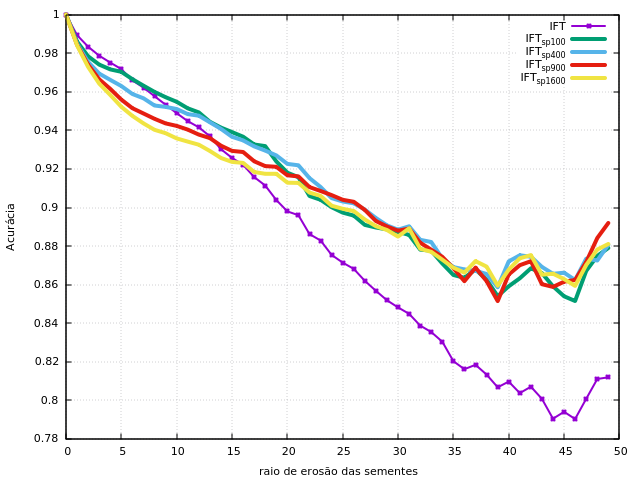
\includegraphics[width=10cm]{figuras/resultados.png}
\caption{\label{fig:resultados} resultados}
\end{center}
\end{figure}



